\documentclass[10pt,a4paper]{article}
\usepackage{amsmath}
\usepackage{amsfonts}
\usepackage{amssymb}
\usepackage{graphicx}
\usepackage{pgfplots}
\pgfplotsset{compat=1.17}
\usepackage{tikz}
\usepackage{float}

\begin{document}

\begin{figure}[H]
    \centering
    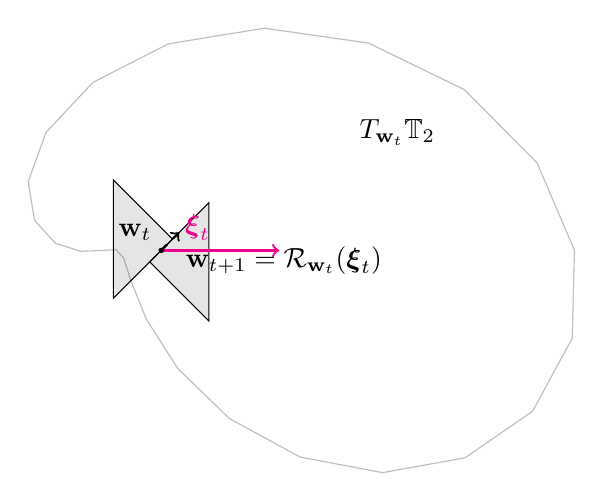
\begin{tikzpicture}[scale=0.75]
        % Torus surface
        \def\r{3}
        \def\R{4}
        \def\ang{60}
        
        \draw[gray, opacity=0.3] plot[domain=0:360, variable=\t] ({(\R+\r*cos(\t))*cos(\t)}, {(\R+\r*cos(\t))*sin(\t)}, {\r*sin(\t)});
        \draw[gray, opacity=0.3] plot[domain=0:360, variable=\t] ({(4+\r*cos(\t))*cos(\t)}, {(4+\r*cos(\t))*sin(\t)}, {\r*sin(\t)});
        
        % Tangent plane
        \draw[fill=black, fill opacity=0.1] 
            (0,0,-0.5) -- (-1,-1,-0.5) -- (-1,1,-0.5) -- (0,0,-0.5);
        \draw[fill=black, fill opacity=0.1] 
            (0,0,0.5) -- (1,-1,0.5) -- (1,1,0.5) -- (0,0,0.5);
            
        % Direction vector
        \draw[->, thick, magenta] (0,0,0) -- node[midway, above left] {$\boldsymbol{\xi}_t$} (2,0,0);
        
        % Retraction arrow
        \draw[->, thick, dashed, black] (0,0,0) -- node[pos=0.8, below right] {$\mathbf{w}_{t+1} = \mathcal{R}_{\mathbf{w}_t} (\boldsymbol{\xi}_t)$} (0.5,0.5,0.5);
        
        % Labels
        \node at (4,2,0) {$T_{\mathbf{w}_t} \mathbb{T}_2$};
        
        % Points
        \filldraw[black] (0,0,0) circle (1pt) node [above left] {$\mathbf{w}_t$};
        
    \end{tikzpicture}
    \caption{Illustration of Riemannian optimization on $\mathbb{T}_2$ (a torus embedded in $\mathbb{R}^3$): the iterate $\mathbf{w}_{t+1}$ is obtained from the retraction $\mathcal{R}_{\mathbf{w}_t}$ applied to the direction descent $\boldsymbol{\xi}_t \in T_{\mathbf{w}_t}\mathbb{T}_2$ (a vector of the tangent space of $\mathbb{T}_2$ at point $\mathbf{w}_t$).}
    \label{fig:tangent_space_torus}
\end{figure}

\end{document}